\documentclass[12pt,letterpaper]{article}

\usepackage{amsmath, amsthm, amsfonts, amssymb}
\usepackage{microtype, parskip, graphicx}
\usepackage[comma,numbers,sort&compress]{natbib}
\usepackage{lineno}
\usepackage{longtable}
\usepackage{docmute}
\usepackage{caption, subcaption, multirow, morefloats, rotating}
\usepackage{wrapfig}
\usepackage{hyperref}

\frenchspacing

\begin{document}

\section{Introduction}

How predictable is extinction? Forecasting species survival at million-year timescales.

One of the great promises of paleobiology is that by studying the past we can better predict the future.  This promise is particularly pertinent given as risk assessments for some modern species could potentially be improved by examining past extinction patterns and by using paleontological records to establish geographic range and abundance trajectories on geological timescales.  Any effort to assess future risk based on past extinctions and range trajectories must address two key questions:  (1) At a given timescale, are geographic range and extinction risk trajectories deterministic (past trends are likely to continue into the future) or Markovian (the future depends only on the present state)? (2) Given knowledge of past extinction/survival patterns and the present geographic ranges of extant taxa, how accurate are extinction risk predictions?  

To address these questions we analyze the fossil record of Cenozoic planktonic microfossil taxa (foramanifera, radiolarians, diatoms, and calcareous nanoplankton). Using a model of species survival, we analyzed how survival probability changes over time as a function of species age, time of observation, current geographic range, most recent change in geographic range, global temperature average, and the lag of global temperature. Our best supported model includes the historical covariates, change in geographic range and lag of global temperature, which indicates that the past improves our estimates of the present and future. 

The effects of the historical covariates are extremely small and vary considerably over time. For example, the effect of change in geographic range size can either increase or decrease probability of extinction depending on when in the Cenozoic the observation takes place. The improvement in predictive power by including these historical covariates is modest at best and reflects the rarity of extinction events (i.e. class-imbalance) and the extremely stochastic nature of species survival. Correcting for class imbalance, we find that in-sample model performance measures are approximately equal to out-of-sample performance as estimated from cross-validation. These results reflect the difficulty of estimating species extinction, and that while including historical covariates does improve model performance, that gain is very small.  This result implies that at million-year timescales geographic range trajectories are nearly Markovian, perhaps because the processes driving geographic range changes vary on substantially shorter timescales. The effect of change in geographic range on survival most likely stands for many interacting and unobserved processes which in-turn produce that species' geographic range and its affect on survival. 

Finally, we find support for species' extinction risk increases with age, though the strength of this effect varies among taxonomic groups. This effect is most pronounced in forams and radiolarians, and less pronounced in diatoms and calcareous nanoplankton. The greatest source of variance in survival probability is the timing of observation. Importantly, this result means that the time of an observation is a greater source of variation in survival probability when compared to species age. 

Ultimately, we find that including information on a species' change in geographic range size on average improves our predictions of species survival at million-year timescales. However, the effect of change in geographic range is much smaller than the effect of current geographic range, and highly variable through time as the effect changes sign and there are times where there is little evidence for any effect of past geographic range. The results of this study reinforce the importance of the promise of paleontology and using the past to predict the future.



Species global geographic range changes over time due to both local and global processes.

An old assumption in paleobiology was that species quickly obtained their maximum global geographic range and then maintained that range till their decline eventual extinction. Observation of species distribution records does not support this assumption. Instead, changes to a species' global geographic range is currently theorized to follow one of two general patterns: hat or hump PERFECT TIME FOR A FIGURE. Both are symmetric patterns but have different shapes. The hat pattern is characterized by an increase in geographic range for the first half a species' duration followed by a brief peak in geographic range, and the a decrease in geographic range for the second half of that species' duration. The hump pattern is instead characterized by a brief period of increasing species geographic range, an extended period of that species' duration at its maximum geographic range, and finally a quick decline and extinction of the species.

\begin{figure}[ht]
  \centering
  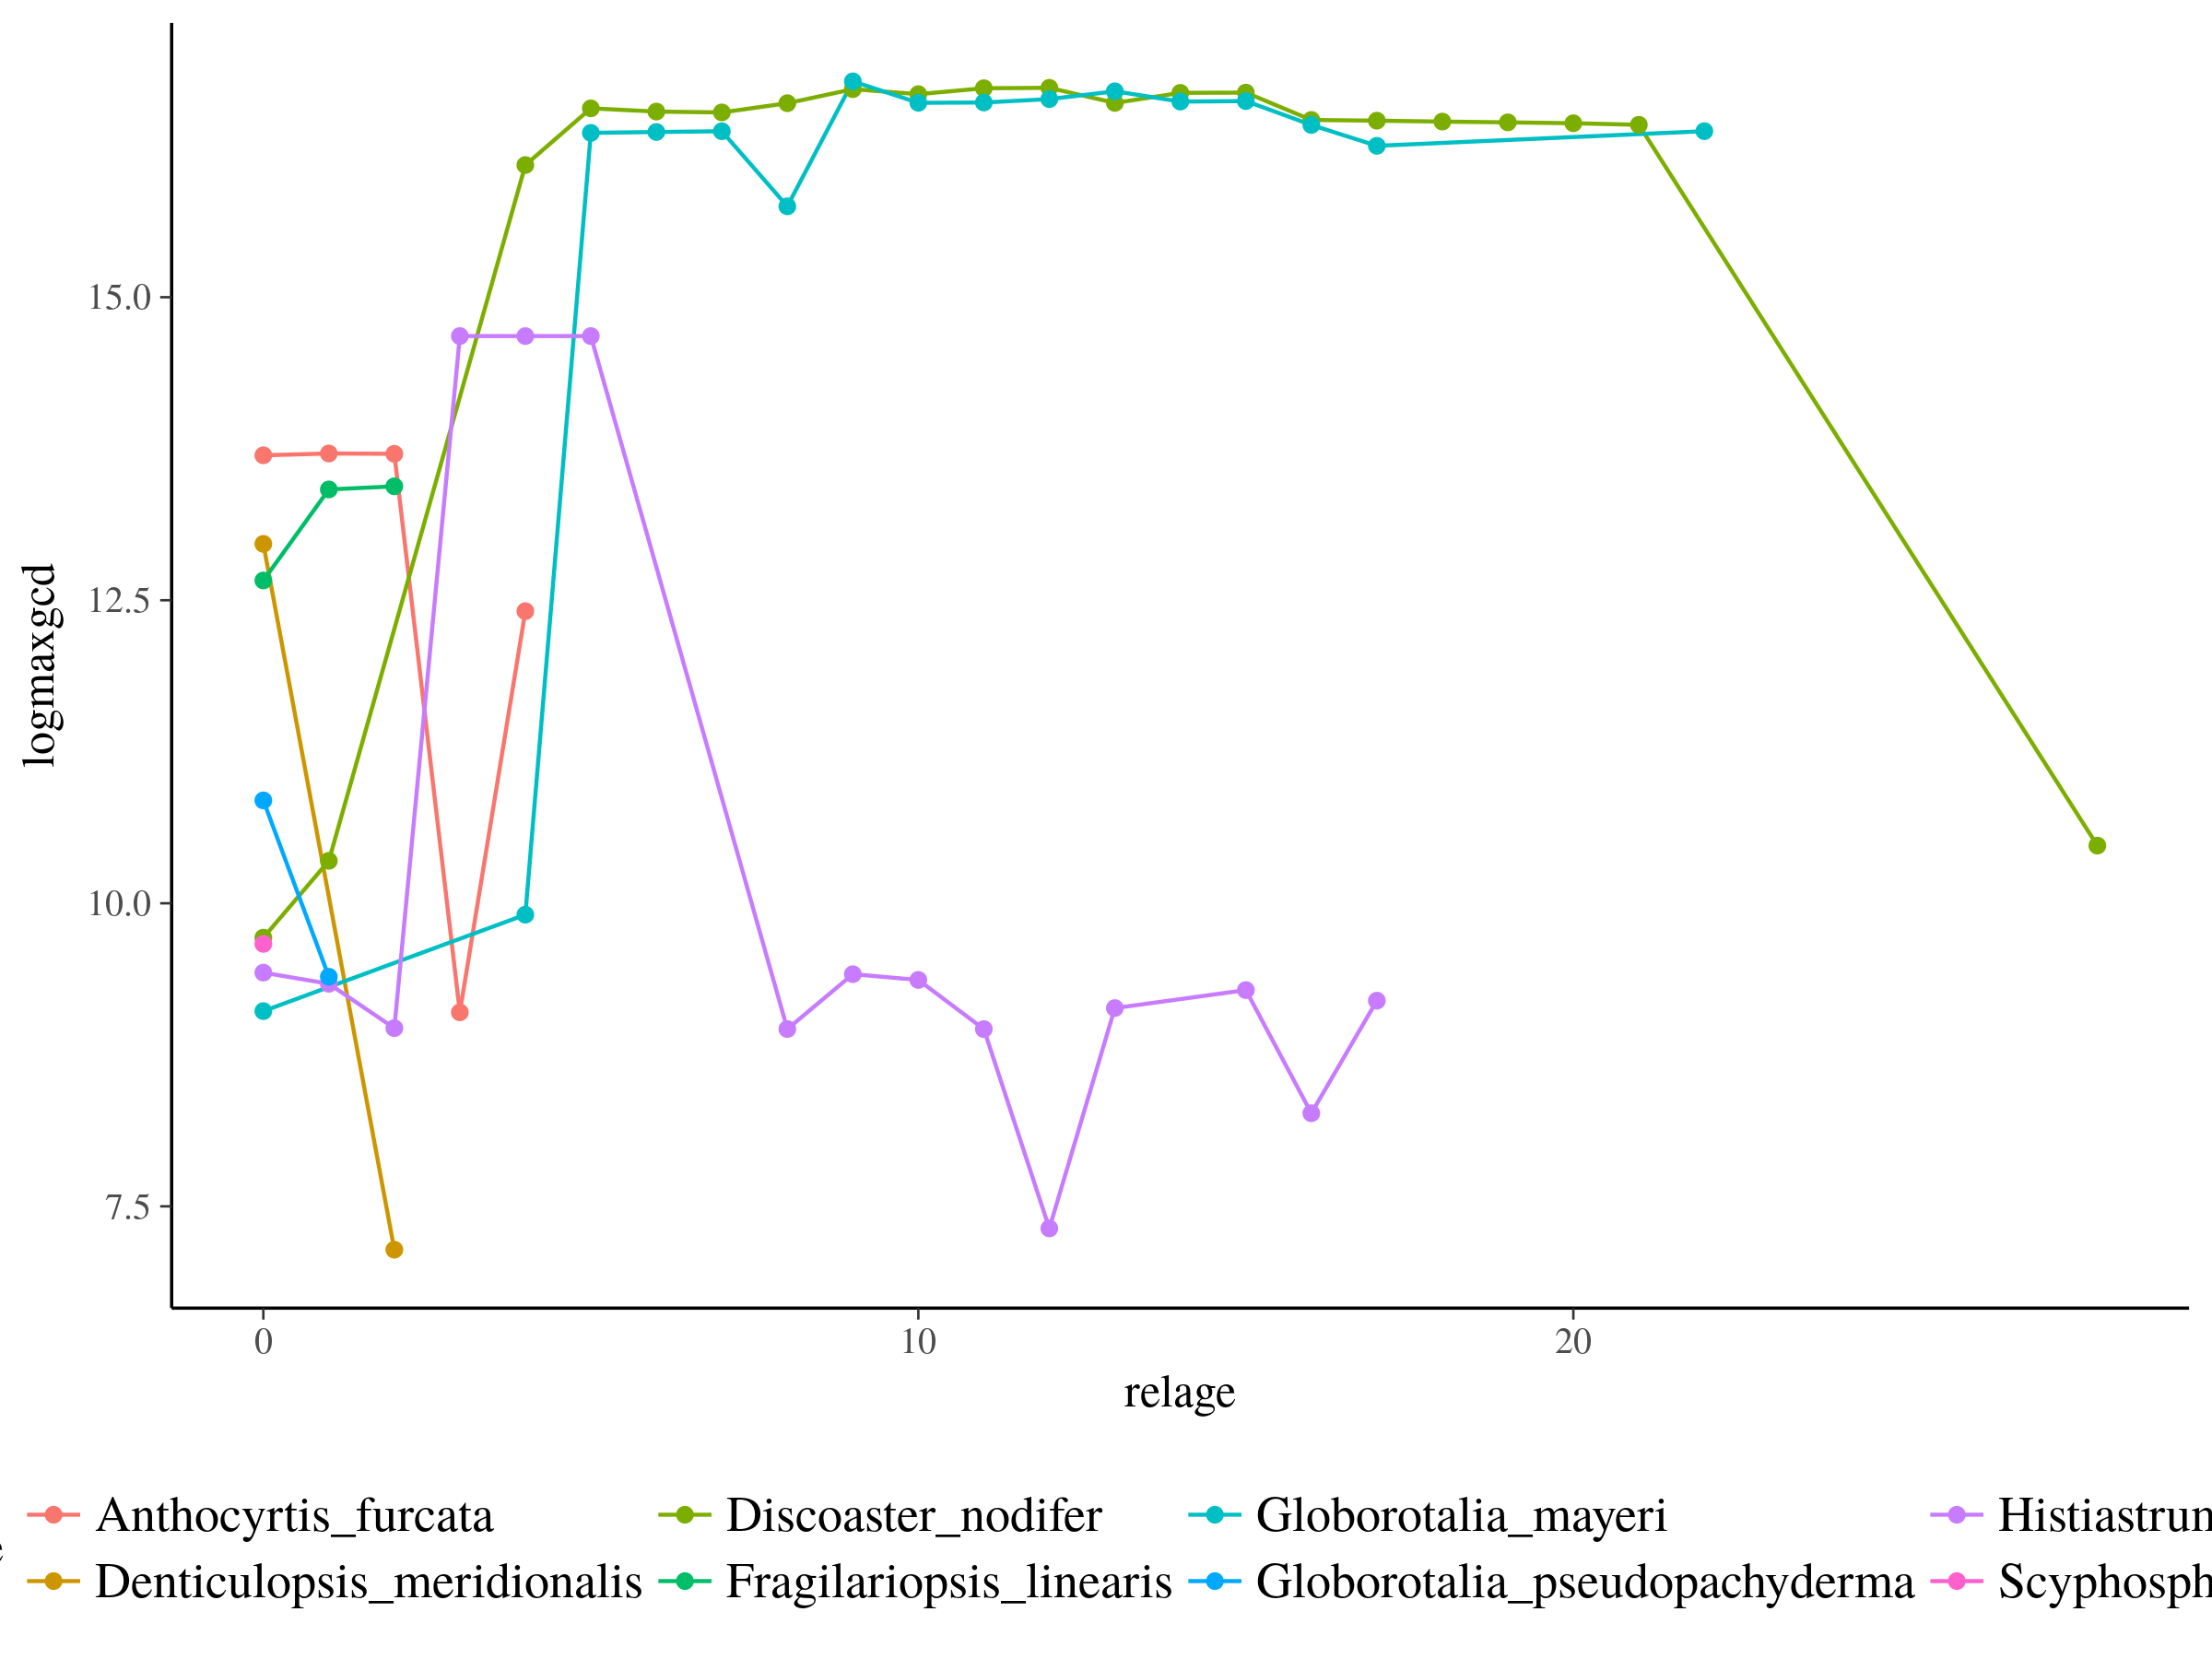
\includegraphics[width=\textwidth,height=0.5\textheight,keepaspectratio=true]{figure/range_time}
  \caption{Geographic range over time for a selection of eight random species included in this analysis. Geographic range is measured as the maximum geodesic distance between two occurrences of that species during a given time interval. The time axis corresponds to species age in millions of years (My). Because each species has a different duration, not all of these trajectories are of equivalent duration.}
  \label{fig:range_real}
\end{figure}

Measuring this pattern is extremely difficult for multiple reasons. Species are not observed continuously through time, species geographic ranges are based on what samples are available, and species are harder to observe at the tails of their duration because they are rare (small geographic range, small population sizes).

Additionally, neither of these patterns are necessarily different from a Markovian process with a lower bound. A random walk beginning at 0 will most likely be unimodal with a period of increase followed by a period of decrease and then eventually reaching 0. This can be demonstrated through a simple simulation PERFECT PLACE FOR A SIMULATION. 

Our simulations are of a random walk with a lower bound of 0. Each individual simulation begins with a value of 0, and for each time step that value is modified by a single realization from a standard Normal distribution. Each simulation had a maximum of 100 time steps beyond the initial point. For each simulation, the first time the value is less than or equal to 0 is considered the stopping point, with that last value set to 0. We retained all simulations which returned to 0, which would be the equivalent of a species going extinct. While we attempted 1000 simulations, not all of these fulfilled this criteria as they did not had a value greater than 0 at their final time step. Finally, the duration of all simulations was rescaled to be between 0 and 1 so that their trajectories are directly comparable. A binned average and moving-window average are calculated from the population of simulations. 

The binned average and moving-window averages are nearly identical to figure 1 from the original rise-and-fall paper by Foote et al. The results from these simulations show that for a random walk bounded at 0, the average trajectory is symmetrical and virtually identical to either the ``hat'' or ``hump'' models and was generated without any deterministic process; the pattern is unimodal and intermediate between ``strict'' hat or hump models. Thus, a hat or hump trajectory demonstrates nothing about process or determinism but could just result from entirely stochastic processes.

 \begin{figure}[ht]
  \centering
  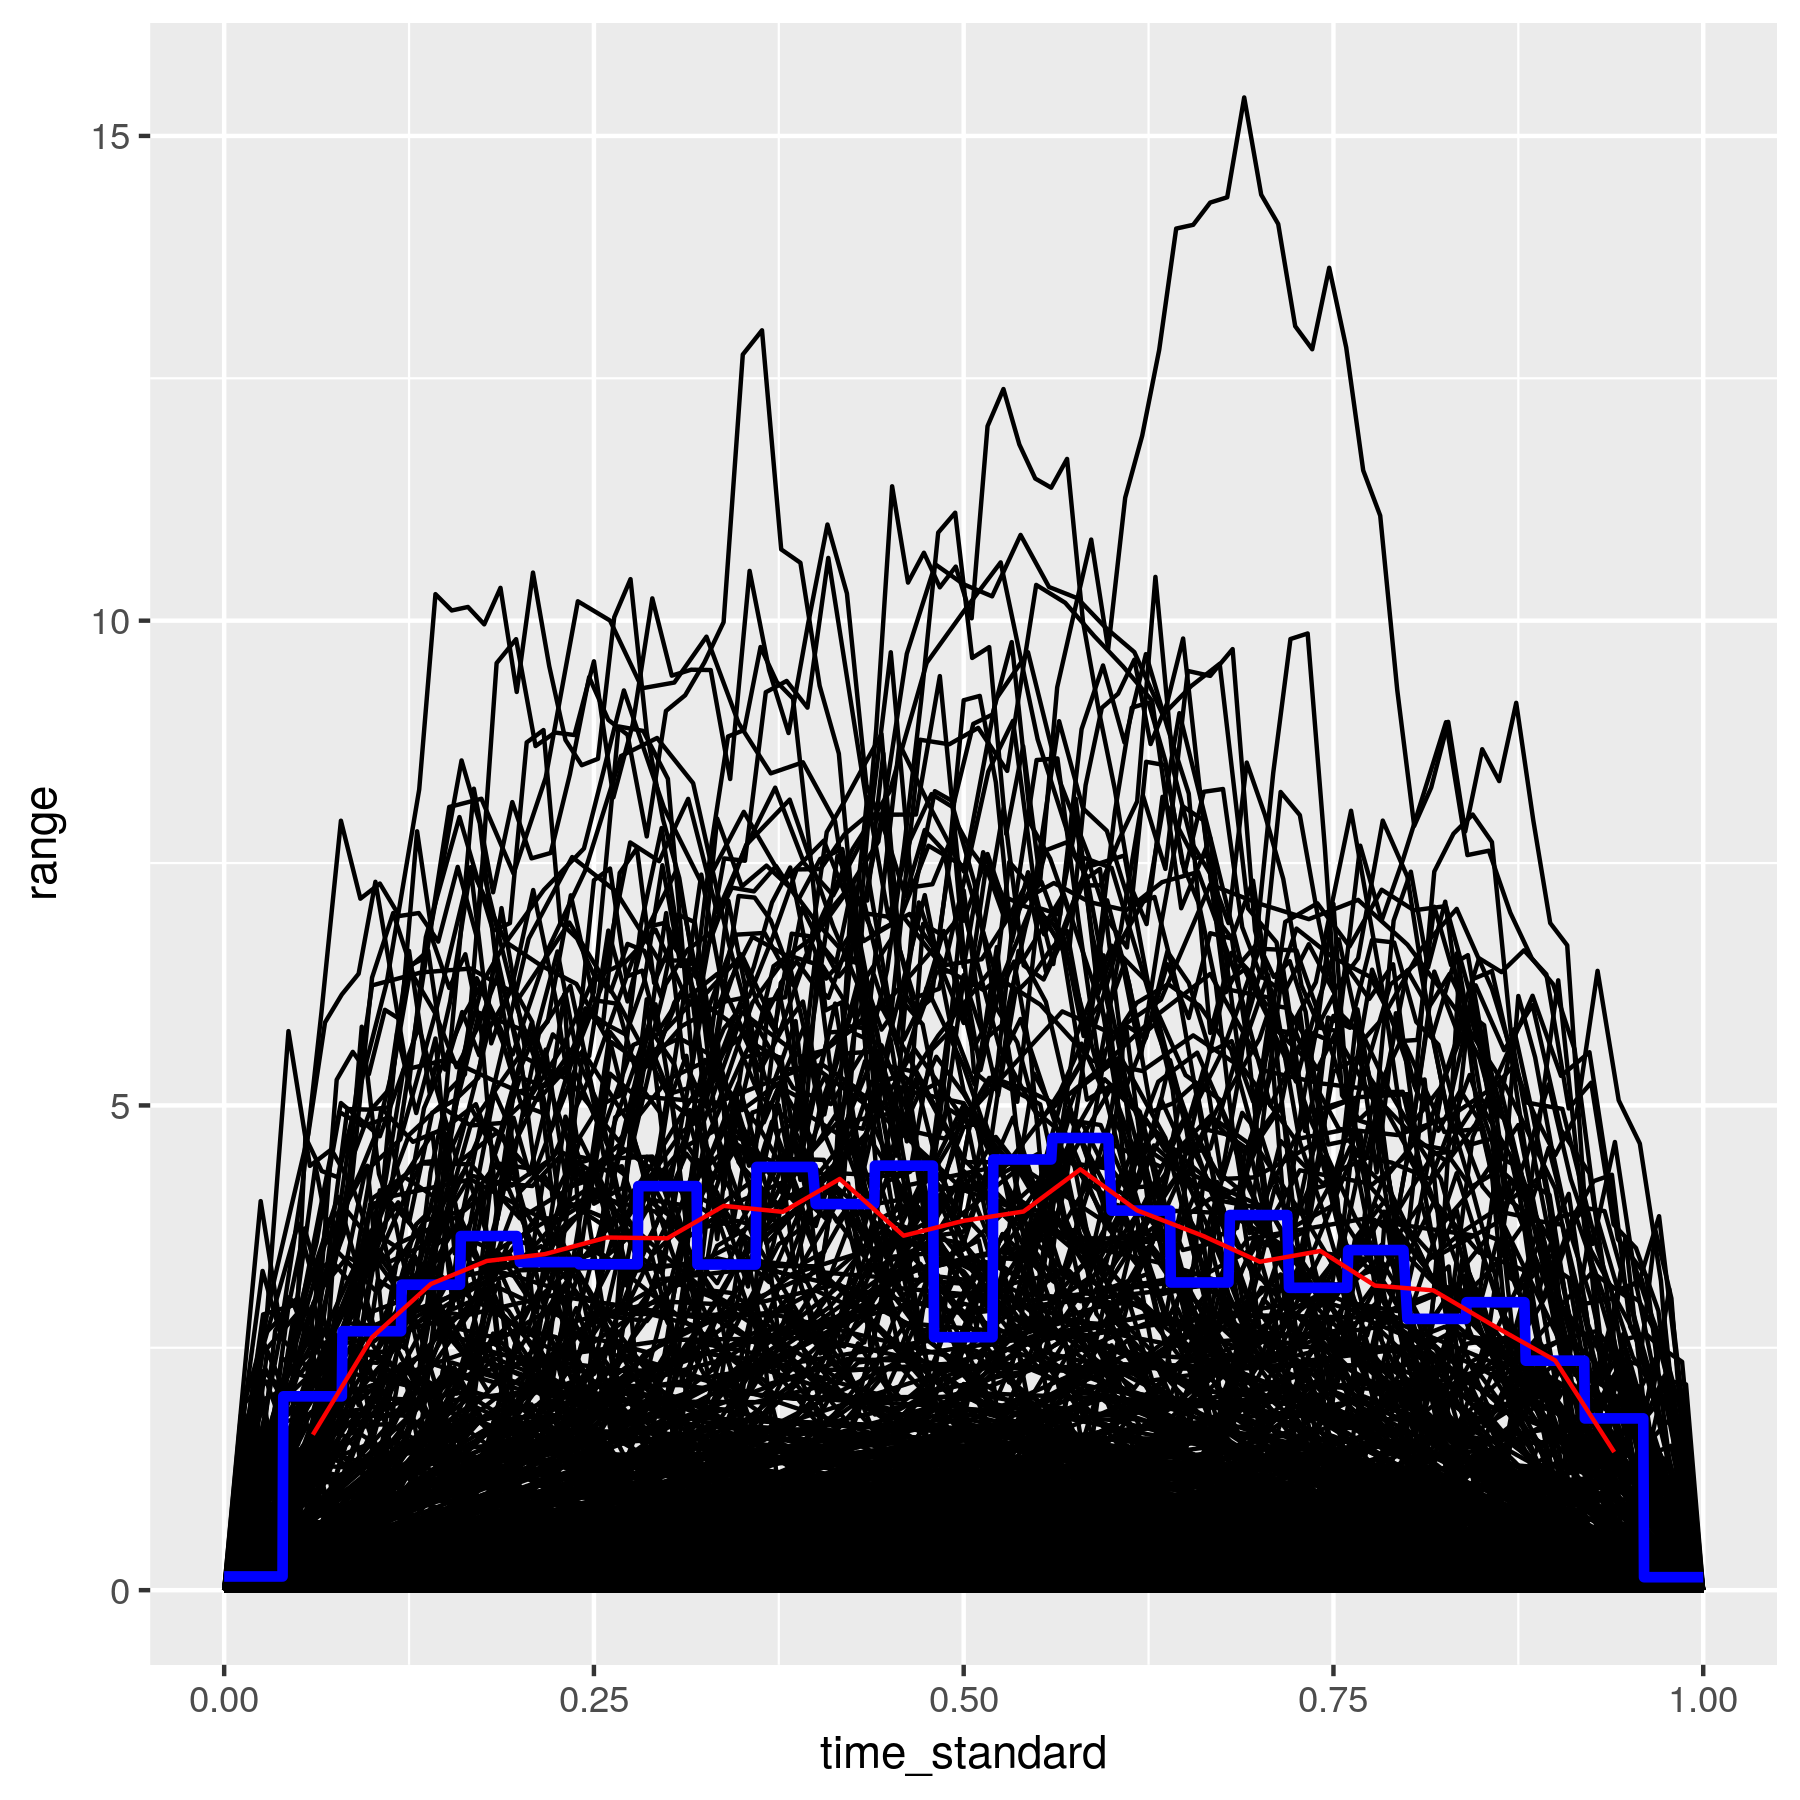
\includegraphics[width=\textwidth,height=0.5\textheight,keepaspectratio=true]{figure/georange_sim_norm}
  \caption{Simulation of a bounded random walk. The blue line is a binned average of all simulations while the red line is a moving-window average of those averages.}
  \label{fig:range_sim}
\end{figure}

Instead of modeling geographic range through time, we instead model extinction probability as a function of change in geographic range. This formulation means that, if there if geographic range trajectory is deterministic and not entirely Markovian, that past geographic range, specifically the change in geographic range, and not just current geographic range predicts the probability of extinction. For example, is extinction probability affected by a species has been decreasing in geographic range over time or does it just matter if that species has below average geographic range regardless of how it got there?





\end{document}
